\documentclass[10pt,a4paper]{article}
\usepackage[utf8]{inputenc}
\usepackage[italian]{babel}
\usepackage{amsmath}
\usepackage{amsfonts}
\usepackage{amssymb}
\usepackage{graphicx}
\usepackage{siunitx}
\usepackage[left=2cm,right=2cm,top=2cm,bottom=2cm]{geometry}
\newcommand{\rem}[1]{[\emph{#1}]}
\newcommand{\exn}{\phantom{xxx}}

\author{Gruppo 1.BN \\ Massimo Bilancioni, Alessandro Foligno, Giuseppe Zanichelli }
\title{Amplificatore a transistor}


\begin{document}

\date{4 ottobre 2018}
\maketitle

\section{Risposta a segnali sinusoidali di frequenza fissa}

Abbiamo scelto una frequenza di lavoro intorno ai $7.40$ \si{\kilo\hertz}.

a) 
\vspace{0.5cm}

i)  Abbiamo verificato l'inversione di fase per VOUT, la figura sotto riporta quanto osservato.

\begin{figure}[h]
	\centering
	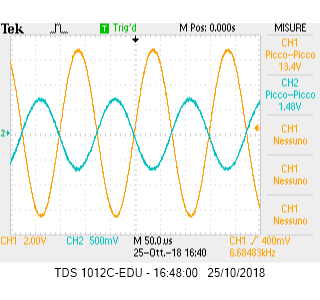
\includegraphics[scale=0.5]{oscilloscopio.png}

	
	
\end{figure}

ii)  Facendo una media dei guadagni per piccole  ampiezze diverse di VIN, otteniamo :\[A_v= (9.76\pm0.01) \]
  (VIN e VOUT sono stati misurati sui due canali differenti dell'oscilloscopio,per questo abbiamo considerato gli errori scorrelati)
\begin{table}[h]
	\centering
	\begin{tabular}{|c|c|c|}
		\hline 
		 VIN (\si{\volt}) &  VOUT (\si{\volt})   & VOUT/VIN\\
		\hline 
	$0.228 \pm  0.06 $& $2.20\pm 0.06$& $9.65 \pm 0.04$\\
	$0.320\pm 0.08 $& $3.12 \pm 0.08$& $9.75 \pm0.04$\\
	$0.528\pm 0.015 $& $5.14 \pm 0.15$& $9.73\pm 0.04$ \\
	$0.752\pm 0.021$& $7.32\pm 0.21$ & $9.73\pm 0.04$\\
	$1.02\pm 0.03 $& $10.2\pm 0.3$& $10\pm 0.04 $\\
	$1.27\pm 0.04$ & $12.3\pm 0.4 $& $9.69\pm 0.04 $\\

		\hline 
	\end{tabular} 
\end{table}

\begin{figure}[h]
	\centering
	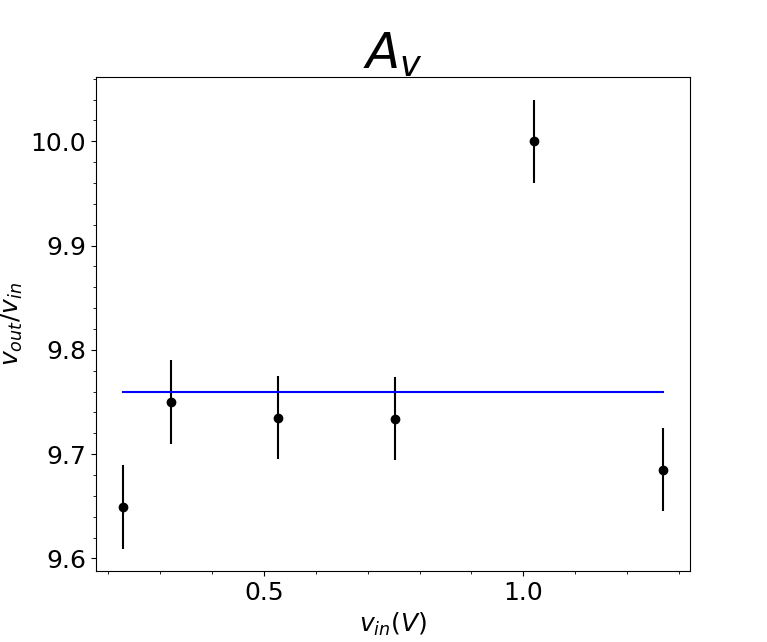
\includegraphics[scale=0.5]{guadagno.png}

	
	
\end{figure}

iii) Per un segnale in ingresso di circa $1.60$ \si{\volt}pp si iniziano a vedere distorsioni per VOUT.

iv)\begin{figure}[h]
	\centering
	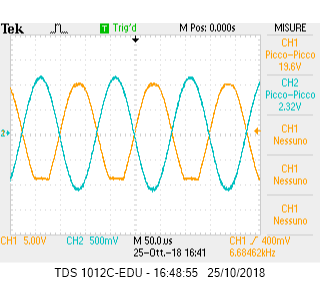
\includegraphics[scale=0.5]{clipping.png}
\end{figure}
\section{Diagramma di Bode}
 Campionando in un intervallo di frequenze che spazia da 1\si{\hertz} a 1\si{\kilo\hertz}, abbiamo costruito un diagramma di Bode del guadagno. I punti sperimentali sono riportati in seguito.
 \begin{figure}[h]
 	\centering
 	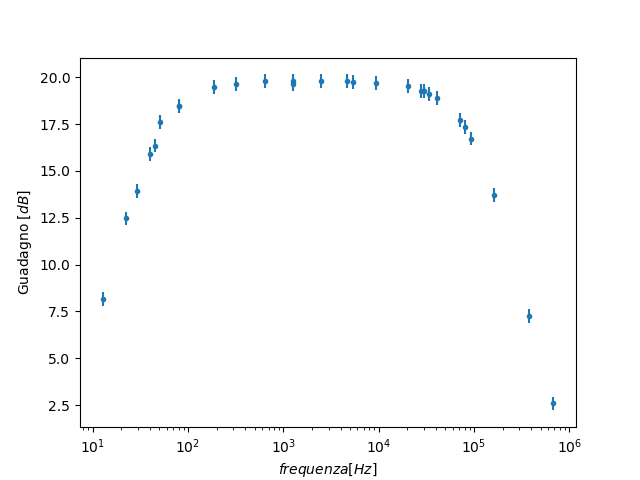
\includegraphics[scale=0.5]{dataBodeplot.png}
	
	
\end{figure}
Visivamente l'andamento sembra quello tipico di un passabanda, eppure, oltre alla traslazione del guadagno massimo (che in questo caso è > 1, grazie al transistor), l'andamento asintotico ai due estremi non è di $\pm 20 dB/Decade$, come nel caso di passa basso e alto in cascata, bensì di circa $-15 \pm0.3dB/Decade $ per basse frequenze e $ 17.7\pm0.2 dB/Decade$ per alte frequenze.
Questi numeri sono ottenuti da fit lineari nelle tre regioni:
\begin{figure}[h]
	\centering
	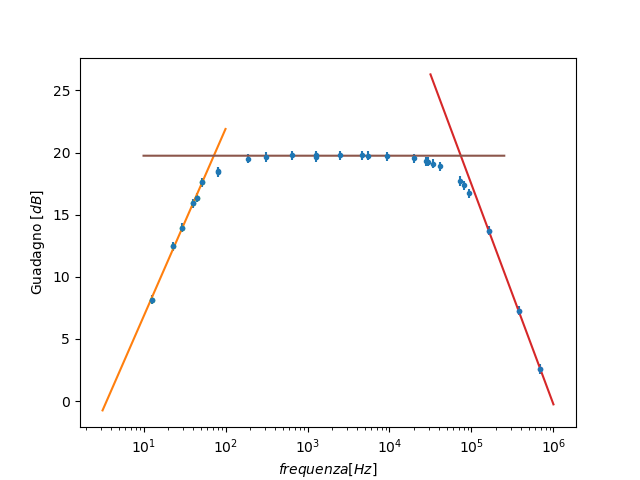
\includegraphics[scale=0.5]{fit.png}
\end{figure}
Lo smorzamento per basse frequenze lo riteniamo dovuto sostanzialmente all'effetto di $C_{IN}$ che si comporta come un passa alto. Trascuro l'effetto di $C_{OUT}$, almeno alle frequenze considerate, dato che $|Z_{oscilloscopio}|\approx1 M\Omega\gg \frac{1}{\omega C_{OUT}}\approx31k\Omega$
Facendo dei conti, si ricava che lo smorzamento è del tipo:\[A=\frac{1}{\sqrt{1+(f_t/f)^2}}\] con $f_t=(2\pi R_{eq} C_{IN})$ e $R_{eq}$ è il parallelo fra R1,RE + la resistenza dinamica del diodo, R2.
Tuttavia l'andamento che segue la curva  non è esattamente, come preannunciato, quello atteso. Questo non può che essere spiegato se non con un aumento del guadagno del diodo per ampiezze più piccole. dato che la diminuzione del guadagno verso basse frequenze è più di quanto attesa.
Viceversa supponiamo che,ad  alte frequenze, l'andamento da passa basso sia dovuto agli effetti induttivi non trascurabili del circuito, ed in particolare della basetta.
Lo smorzamento, di nuovo non è esattamente di $-20 dB/Decade$, supponiamo, di nuovo, a causa del comportamento non lineare del transistor.

\section*{Dichiarazione}
I firmatari di questa relazione dichiarano che il contenuto della relazione \`e originale, con misure effettuate dai membri del gruppo, e che tutti i firmatari hanno contribuito alla elaborazione della relazione stessa.

\end{document}